%--------------------------------------------------------------------------------------------------
%
\chapter{Complexity and Relaxations}\label{sec:crosslingual}
%--------------------------------------------------------------------------------------------------

\subsection{NP-Hardness}\label{subsec:nphard}
In this section, we prove that the optimization problem is not only
non-convex but is NP-hard in general. We use a reduction from a general binary quadratic
optimization problem.
%
%
Let $A   \in \RR^{m\times m}$.  %and $x := (x_1, \ldots, x_m)^T \in \RR^m$.
The binary quadratic optimization problem (BQO) is stated as:
\begin{equation}\label{eq:binqp}
\tag{BQO}
\begin{aligned}
& \underset{x \in \RR^m}{\text{max}}
& & x^T A x  \\
& \text{subject to}
& & x\left(i\right)^2 = 1,  \quad\forall i =1,\ldots,m.\\
\end{aligned}
\end{equation}
Many hard combinatorial optimization problems (e.g. the
maximum cut  problem and the maximum clique problem~\cite{Garey:1990:CIG:574848}) can be reduced to
BQO \cite{Goemans95improvedapproximation}, which is known to be NP-hard.

%\textcolor{red}{a je ocitno da to nice ne spremeni }

We reduce a general instance of a  BQO problem to an
instance of the problem (\ref{eq:qcqp}). That means that despite the special
structure of the
problem (\ref{eq:qcqp}) (maximizing a positive-definite quadratic form over a
product of spheres), it still falls into the class of problems that are hard (under the assumption that $P \neq NP$).
We begin with a general instance of BQO and through a set of simple transformations, obtain a specific
instance of (\ref{eq:qcqp}), with a block structure $b =
\left(1,\ldots,1\right)$. The transformations will turn an arbitrary
BQO matrix $A$ into a correlation matrix, while preserving  the optimal solutions.


 Consider a BQO with a corresponding general matrix $A \in \RR^{m\times m}$. Since $x^T A x = x^T
\frac{\left(A + A^T\right)}{2} x$, we can assume that the matrix $A$ is
symmetric. The binary constraints imply that for any diagonal
matrix $D$ the quantity $x^T D x = \sum_i D\left(i,i\right)$ is
constant. This means that for $c > 0$ large enough, we can
replace the objective with an equivalent objective $x^T \left(A + c
\cdot I\right) x$ which is a positive-definite quadratic form. Setting $c := \norm{A}_1 + 1$ guarantees that $A + c\cdot I$ is positive definite, which follows from strict diagonal dominance. From
now on, we assume that the matrix $A$ in the BQO is symmetric and
positive-definite.  Let $g = \max_i{A\left(i,i\right)}$ and let $D \in
\RR^{m\times m}$ be the diagonal matrix with elements $D\left(i,i\right) = g -
A\left(i,i\right)$. The BQO is then equivalent to
\begin{equation}\label{eq:binqpcor}
\begin{aligned}
& \underset{x \in \RR^m}{\text{max}}
& & x^T \frac{\left(A + D\right)}{g} x  \\
& \text{subject to}
& & x\left(i\right)^2 = 1,  \quad\forall i =1,\ldots,m.\\
\end{aligned}
\end{equation}
The matrix $\frac{\left(A + D\right)}{g}$ is a correlation matrix since it
isa symmetric positive-definite with all diagonal entries
equal to $1$. The optimization problem corresponds to a problem
of maximizing a sum of pairwise correlations between univariate
random variables (using block structure notation: $b\left(i\right) = 1,
\forall i = 1,\ldots, m$). This shows that even the simple case
of maximizing the sum of correlations where the optimal axes are
known and only directions need to be determined, is NP-hard.

With a fixed number of views, the complexity is polynomial, based on results on quadratic maps \cite{Grigoriev}. The degree of the polynomial is asymptotically equal to the product\footnote{The number of local solutions to our problem of interest is established in \cite{Chu}.} $\prod_{i=1}^m n_i$, where $n_i$ is the dimensionality of the $i$-th view.
In many applications (text mining, fMRI analysis) where the $n_i$'s are large the computational cost becomes prohibitive even with $m=3$.

%\textbf{Some discussion on number of views}

\subsection{Local solutions}\label{subsec:horst}
Given the hardness result, a
natural approach is to use local methods to obtain a (possibly suboptimal)
solution.  In this section, we give an algorithm that converges to a locally optimal solutions of the problem (\ref{eq:qcqp}), when the matrix $A$ is symmetric,
positive-definite and generic (the proof was established in \cite{Chu}).

The algorithm can be interpreted as a generalization of the power
iteration method (also known as the Von Mises iteration), a classical
approach to finding the largest solutions to the eigenvalue problem $A
x = \lambda x$.  The general iterative procedure is given as Algorithm~\ref{algorithm:horst}.
\begin{algorithm}
\caption{Horst algorithm}
\label{algorithm:horst}
{\bf Input:} matrix $A \in \sym_N^+$, block structure $b = \left(n_1,\ldots,n_m\right)$, initial vector $x_0 \in \RR^N$ with $\norm{x^{(i)}} > 0$,  \par
\begin{algorithmic}
\STATE $x \leftarrow x_0;$
\FOR{$iter = 1$ to $maxiter$}
\STATE $x \leftarrow A x;$
\FOR{$i =1$ to $m$}
\STATE $x^{(i)} \leftarrow \frac{x^{(i)}}{\norm{x^{(i)}}}$
\ENDFOR
\ENDFOR
\end{algorithmic}
{\bf Output:} $x$
\end{algorithm}
%\STATE $\alpha_j^{i} \leftarrow  \sum_{k}A_{j,k } \alpha_k^{i-1}$
%\STATE $\alpha_j^i \leftarrow \frac{\alpha_j^{i}}{\sqrt{{\alpha_j^i}' \alpha_j^i}}$
% Every step of the main loop in the algorithm \ref{algorithm:horst} involves $m^2$ matrix vector multiplications.
% We can exploit the structure of the problem, namely the fact that the MEP matrix is a sum of block diagonal matrices and a low rank block matrix (with block column matrix as its Cholesky factor) and gain a speed up by a factor of $m$.
In the case of $m=1$,  Algorithm~\ref{algorithm:horst}
corresponds exactly to the power iteration. While the algorithm's
convergence is guaranteed, its convergence rate is not known. In
practice, we observe a linear convergence (Figures~\ref{fig:qcqpConvVar}
and \ref{fig:qcqpConvFix}). In Figure~\ref{fig:qcqpConvVar}, we
generated $1000$ random\footnote{We used the random Gram matrix method
  to generate random problem instances; for details see
  Section~\ref{subsec:syndata}} instances of matrices $A$ with block
structure $b = \left(2,2,2,2,2\right)$. For each matrix, we generated
a starting point $x_0$ and ran the algorithm. The plot depicts the
solution change rate on a logarithmic scale ($log_{10}
\frac{\norm{x_{old} - x}}{\norm{x}}$). We observe linear convergence
over a wide range of rates of convergence (slopes of the
lines). Figure~\ref{fig:qcqpConvFix} shows the convergence properties
for a fixed matrix $A$ with several random initial vectors $x_0$. The
problem exhibits a global
and a local solution. For $65\%$ of the initial vectors, the global solution was reached (versus $35\%$ for the local solution). Note that the global
solution paths tend to converge faster (the average global solution path slope is  $-0.08$, compared  to $-0.05$ for the local solution paths).

%
%\begin{figure*}[htbp]
%  \centering
%\subfigure[Convergence plot ($1000$ random matrices $A$, one random $x_0$ per problem instance)]{\label{fig:qcqpConvVar}
%    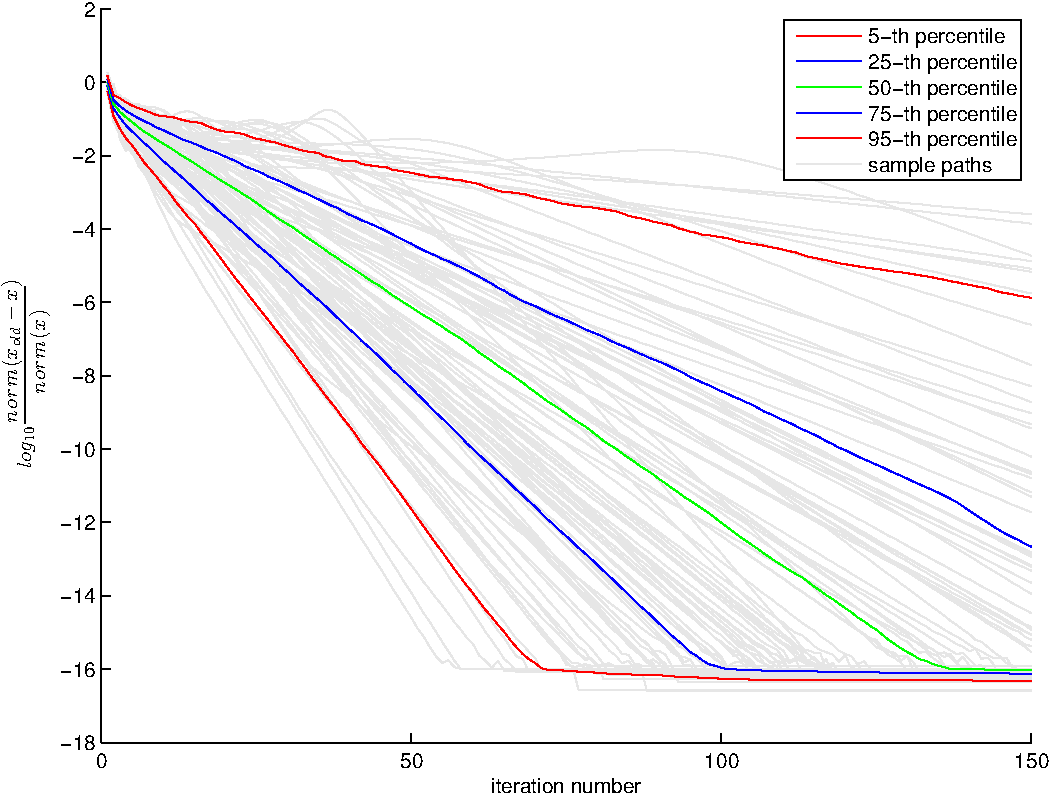
\includegraphics[width=0.47\textwidth]{figures/convergenceBoxPlotDifferentA.pdf}
%}
%\subfigure[Convergence plot (single random $A$, $1000$ random initial vectors $x_0$)]{\label{fig:qcqpConvFix}
%    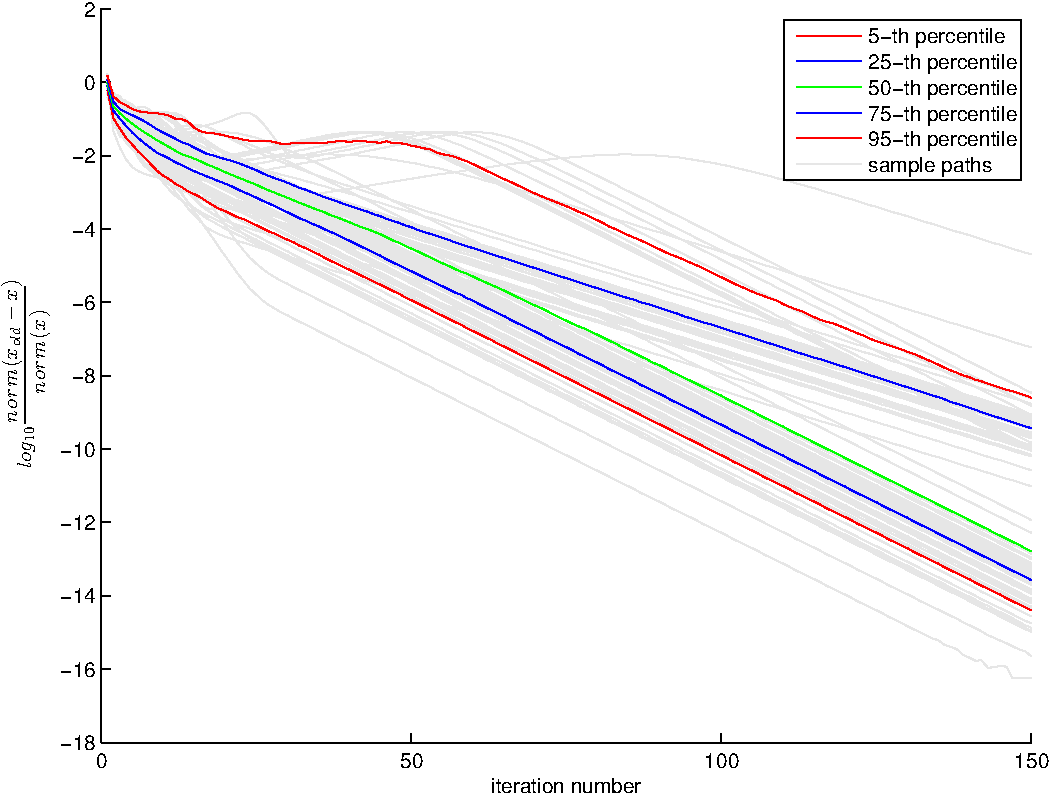
\includegraphics[width=0.47\textwidth]{figures/convergenceBoxPlotFixedA.pdf}
%}
%\end{figure*}

\subsection{Global analysis}\label{subsec:globalanalysis}
The above algorithm is highly scalable and often works well in
practice (see Section~\ref{sec:experiments}).
However, it may not converge to a globally optimal
solution.  We show how to use a relaxation of the problem to obtain
candidate solutions for the original problem. The relaxation
transforms the problem into a  semidefinite program and we
 prove  lower bounds which
relates the extracted SDP solution quality and the optimal QCQP
objective value. We also present a set of upper bounds on the optimal QCQP objective value \ref{subsubsec:upperbounds}.
These can serve as certificates of optimality (or closeness to
optimality) for the local solutions (obtained by the local iterative approach for example).

\subsubsection{Semidefinite programming relaxation}\label{subsubsec:sdp}
%\noindent\textbf{SDP Relaxation}
In this section, we relax  (\ref{eq:qcqp}) to a SDP.
Let $A, B_1, \ldots, B_m  \in \RR^{N \times N}$ be symmetric, positive semidefinite matrices which share the block structure $b := \left(n_1, \ldots, n_m\right), \sum_i b\left(i\right) = N$.
The blocks $B_i^{(k,l)} \in \RR^{n_k \times n_l}$ for $i,k,l = 1,\ldots,m$ are defined as:
$$
B_i^{(k,l)} := \left\{
     \begin{array}{l l}
       I_{n_i} & : k = i, l = i\\
       0_{k,l} & : otherwise
     \end{array}
   \right.,
$$
where $I_{n_i} \in \RR^{n_i \times n_i}$ is an identity matrix and $0_{k,l} \in \RR^{k \times l}$ is a matrix with all entries equal to zero.
Since $x^T A x = \mathrm{Tr}\left( A x x^T\right)$, (\ref{eq:qcqp})
can be rewritten as:
%
\begin{equation}\label{eq:qcqp2}
\tag{QCQP2}
\begin{aligned}
& \underset{x \in \RR^n}{\text{max}}
& &\mathrm{Tr}\left(A x x^T\right) \\
& \text{subject to}
& &\mathrm{Tr}\left(B_i x x^T\right) = 1,  \quad\forall i =1,\ldots,m.\\
\end{aligned}
\end{equation}
%
%
Substituting the matrix $x x^T$ with a general matrix $X \in \sym_{+}^{n}$ constrained to have rank one:
%
\begin{equation*}
\begin{aligned}
& \underset{X \in \sym_{+}^n}{\text{maximize}}
& &\mathrm{Tr}\left(A X\right) \\
& \text{subject to}
& &\mathrm{Tr}\left(B_i X\right) = 1,  \quad\forall i =1,\ldots,m\\
& & &\mathrm{rank}\left(X\right) = 1.
\end{aligned}
\end{equation*}
%
%
%
%\begin{remark}
%Matrices $A$ and $B_1,\ldots,B_m$ are symmetric positive-semidefinite matrices.
%This is obvious for matrices $B_i$ and observe that matrix $A$ is similar to a covariance matrix corresponding to random vector $(X_1',\ldots, X_m')'$, hence positive-semidefinite.
%\end{remark}
%
Omitting the rank-one constraint, we obtain a semi-definite program in standard form:
%
\begin{equation}\label{eq:sdp}
\tag{SDP}
\begin{aligned}
& \underset{X \in \sym_{+}^n}{\text{max}}
& &\mathrm{Tr}\left(A X\right) \\
& \text{subject to}
& &\mathrm{Tr}\left(B_i X\right) = 1,  \quad\forall i =1,\ldots,m.\\
\end{aligned}
\end{equation}
%
%\begin{remark}
%If the solution of the problem (\ref{eq:sdp}) is rank-one, i.e. $X$ can be expressed as $X = y \cdot y^T$, then $y$ is the optimal solution for (\ref{eq:qcqp}).
 %for $y = (y_1^T, \ldots, y_m^T)^T\in \RR^{N}$, where $y_i \in \RR^{n_i}$ are block components of vector $y$, then a solution to the problem (\ref{eq:qcqp}) is obtained by setting $x_i = y_i$.
%\end{remark}
%
%
\noindent\textbf{Low rank solutions}
We use the solutions of the SDP relaxation to extract solutions to
the original QCQP problem. In the process, we obtain a bound which relates
the global SDP bound and the optimal value of QCQP, giving a measure of
the quality of the extracted solution. If the solution is
rank-one, then the relaxation is exact. Here we consider the case where the solutions are
 low rank(close to rank-one).

Let $X^*$ be a solution to (\ref{eq:sdp}) and $x^{*}$ be the solution
to (\ref{eq:qcqp}).
A straightforward way to extract a feasible solution to the problem
(\ref{eq:qcqp}) from $X^*$ is to project its leading eigenvector to
the set of constraints.  The following inequality always holds:
 $$\mathrm{Tr}\left(A X^{*}\right) \geq \mathrm{Tr}\left(A \cdot x^{*} \cdot x^{*T}\right).$$
The quality of the solution depends on how loose this inequality is,
or rather how close the matrix $X^*$ is to rank-one (Proposition \ref{thm:rank2sdp_solution}). These depend on the spectral properties of matrix
$X$ and matrix $A$.
 %
%
 %Let $b = \left(n_1,\ldots,n_m\right), \sum_i
%n_i = N $ denote the block structure.
%

The projection of a vector $y \in \RR^N, \norm{y^{(i)}} \neq 0$ to the feasible set of (\ref{eq:qcqp}) is:
% is given by map $\pi\left(\cdot\right) : \RR^N \rightarrow \RR^N$:
$$\pi\left(y\right) := \left(\frac{y^{(1)}}{\norm{y^{(1)}}}, \ldots, \frac{y^{(m)}}{\norm{y^{(m)}}}\right)^T.$$
%Our theorems
We require the following technical assumption:
\begin{assumption}\label{thm:assumption1}
Let $b = \left(n_1,\ldots,n_m\right)$ denote the block structure and $ \sum_i n_i = N $.
Let $X^*$ be the solution to the problem (\ref{eq:sdp}). Let $x_k$ denote the $k$-th eigenvector of $X^*$.
The assumption is the following: $$\norm{x_1^{(i)}} > 0, \forall i = 1,\ldots, m.$$
\end{assumption}
\begin{conjecture}\label{thm:conj1}
Assumption \ref{thm:assumption1} holds in general for optimal solutions to  the problem (\ref{eq:sdp}).
\end{conjecture}
The assumption ensures that the projection to the feasible set,
$\pi(\cdot)$, is  well defined. In our experiments, this was always
the case, but we have been unable to find a proof. %The result that we
%will state after
The following lemma depends on the projection
operator and thus relies on the assumption.
%
\begin{lemma}
Let $b = \left(n_1,\ldots,n_m\right)$ denote the block structure and $ \sum_i n_i = N $.
Let $X^*$ be the solution to (\ref{eq:sdp}).
Let $x_k$ denote the $k$-th eigenvector of $X^*$.
Let $\alpha_i := \frac{1}{\norm{x_1^{(i)}}}$.
If $X^*$ can be expressed as:
$$X^* = \lambda_1  x_1 x_1^T + \lambda_2 x_2 x_2^T,$$
where $x_1$ and $x_2$ have unit length and $\lambda_1 > 1 >  \lambda_2$, then
$$\lambda_1 \leq \alpha_i \alpha_j  \leq \frac{\lambda_1}{1 - \lambda_2}.$$
\end{lemma}
%
\begin{proof}
The constraints in problem (\ref{eq:sdp}) are equivalent to:
$$\lambda_1 \norm{x_1^{(i)}}^2 + \lambda_2 \norm{x_2^{(i)}}^2 = 1, \forall i = 1,\ldots, m.$$
Since $\lambda_2 < 1$ and $\norm{x_2^{(i)}}^2 \leq 1$, we see that $0 \leq \lambda_2 \norm{x_2^{(i)}}^2  < 1$.
Consequently:
$$  0 < \frac{1- \lambda_2}{\lambda_1} < \norm{x_2^{(i)}}^2 \leq \frac{1}{\lambda_1}.$$
From $\alpha_i = \frac{1}{x_1^{(i)}}$ it follows that $$ \sqrt{\lambda_1} \leq \alpha_i \leq \sqrt{\frac{\lambda_1}{1-\lambda_2}},$$
and finally:
$$ \lambda_1 \leq \alpha_i \alpha_j \leq \frac{\lambda_1}{1-\lambda_2}, \forall i,j = 1,\ldots,m.$$
%\qed
\end{proof}
%
\begin{proposition}\label{thm:rank2sdp_solution}
Let $b = \left(n_1,\ldots,n_m\right)$ denote the block structure and $ \sum_i n_i = N $.
Let $X^*$ be the solution to (\ref{eq:sdp}) and $x^{*}$ be the solution to  (\ref{eq:qcqp}).
Let $x_k$ denote the $k$-th eigenvector of $X^*$, $\alpha_i := \frac{1}{\norm{x_1^{(i)}}}$,
$\psi := \mathrm{Tr}\left(A X^{*}\right)$, and $\phi := \mathrm{Tr}\left(A \cdot x^{*} \cdot x^{*T}\right)$.
%$\pi(OP_3) := \mathrm{trace}(A \cdot \pi(x_1) \cdot \pi(x_1^T)$.
If $X^*$ can be expressed as
$$X^* = \lambda_1  x_1 x_1^T + \lambda_2 x_2 x_2^T,$$
where $x_1$ and $x_2$ have unit length and $\lambda_1 > 1 >  \lambda_2$,
 then: $$\psi - \pi\left(x_1\right)^T A \pi\left(x_1\right) \leq  \left(\frac{1}{1-\lambda_2} -1\right)  m^2 + \lambda_2 \norm{A}_2.$$
\end{proposition}
%
\begin{proof}
First we note that: $$\psi \geq \phi \geq \pi\left(x_1\right)^T A \pi\left(x_1\right).$$ We can expand the left hand side in terms of the two eigenvectors. Grouping the elements by the vector terms and using basic manipulations we arrive at the result.
\begin{align*}
\psi &- \pi\left(x_1\right)^T A \pi\left(x_1\right) = \lambda_1 \sum_{i,j} x_1^{(i)T} A^{(i,j)} x_1^{(j)T}  + \\
+ &\lambda_2\sum_{i,j} x_2^{(i)T} A^{(i,j)} x_2^{(j)T} - \sum_{i,j} \alpha_i \alpha_j x_1^{(i)T} A^{(i,j)} x_1^{(j)T}  \leq \\
&\leq  \sum_{i,j} (\lambda_1 - \alpha_i \alpha_j) x_1^{(i)T} A^{(i,j)} x_1^{(j)T}  + \lambda_2 \norm{A}_2 \leq\\
&\leq -\sum_{i,j} (\lambda_1 - \alpha_i \alpha_j)\cdot |x_1^{(i)T} A^{(i,j)} x_1^{(j)T}| +  \lambda_2 \norm{A}_2 \leq\\
&\leq \left(\frac{\lambda_1}{1-\lambda_2} - \lambda_1 \right)\cdot \sum_{i,j}  \frac{1}{\alpha_i \alpha_j} +  \lambda_2 \norm{A}_2 \leq\\
&\leq \left(\frac{\lambda_1}{1-\lambda_2} - \lambda_1 \right)\cdot \frac{m^2}{\lambda_1} +  \lambda_2 \norm{A}_2 =\\
&= \left(\frac{1}{1-\lambda_2} - 1 \right)\cdot m^2 +  \lambda_2 \norm{A}_2.
\end{align*}
%\qed
\end{proof}
%
A similar bound can be derived for the general case, provided that the solution to problem (\ref{eq:sdp}) is close to rank-one.
\begin{proposition}
Let $b = \left(n_1,\ldots,n_m\right)$ denote the block structure and $ \sum_i n_i = N $.
Let $X^*$ be the solution to the problem (\ref{eq:sdp}) and $x^{*}$ the solution to the problem (\ref{eq:qcqp}).
Let $x_k$ denote the $k$-th eigenvector of $X^*$,
$\alpha_i := \frac{1}{\norm{x_1^{(i)}}}$ and
$\psi := \mathrm{Tr}\left(A X^{*}\right)$. %, $\phi := \mathrm{trace}(A \cdot x^{*} \cdot x^{*T})$.
%Let $a_i := \frac{1}{\norm{x^{(i)}_1}}$ and let $OP_3 := \mathrm{trace}(A X^{*})$, $OP_2 := \mathrm{trace}(A \cdot x^{**} \cdot x^{**'})$ and
%$\pi(OP_3) := \mathrm{trace}(A \cdot \pi(x^{(1)}) \cdot \pi(x^{(1)})')$.
If $X^*$ can be expressed as
$$X^* = \lambda_1  x_1 x_1^T + \lambda_2 x_2 x_2^T + \cdots + \lambda_n x_n x_n^T,$$
where each $x_i$ has unit length and $\lambda_1 > 1 >  \underset{i=2,\ldots, n}{\sum} \lambda_i$,
 then:
\begin{align*}
\psi &- \pi\left(x_1\right)^T A \pi\left(x_1\right) \\ &\leq  \left(\frac{1}{1- \underset{i=2,\ldots, n}{\sum} \lambda_i} -1\right)  m^2 + \left(\underset{i=2,\ldots, n}{\sum} \lambda_i\right) \norm{A}_2.
\end{align*}
\end{proposition}


\subsubsection{Upper bounds on QCQP}\label{subsubsec:upperbounds}
We now present several upper bounds on the optimal QCQP objective
value based on the spectral
properties of the QCQP matrix $A$. We then bound the
values of the SDP solutions and present two constant relative accuracy
guarantees.

\noindent\textbf{$\mathbf{L_2}$ norm bound}
We show an  upper bound on the objective of (\ref{eq:qcqp}) based on the largest eigenvalue of the problem matrix $A$.
%
\begin{proposition}
The objective value of (\ref{eq:qcqp}) is upper bounded by $m \cdot \norm{A}_2$.
\end{proposition}
\begin{proof}
The problem (\ref{eq:qcqp}) remains the same if we add a redundant constraint $x^T x = m$ obtained by summing the constraints $\sum_{i= 1}^{m} \left(x^{(i)T}x^{(i)} - 1\right) = 0$. We then relax the problem by dropping the original constraints to get:
\begin{equation}\label{eq:evp}
\begin{aligned}
& \underset{x \in \RR^{N}}{\text{max}}
& & x^T A x\\
& \text{subject to}
& &x^{T} x = m.
\end{aligned}
\end{equation}
Since $\norm{A}_2 = \text{max}_{\norm{x}_2 = 1} x^T A x$, it follows that the optimal objective value of the problem (\ref{eq:evp}) equals $m \cdot \norm{A}_2 $.
\end{proof}
%
\noindent\textbf{Bound on possible SDP objective values}
The next lemma establishes two simple bounds on the optimal value of the SDP problem.
\begin{lemma}\label{eq:lemsdp}
Let $X^*$ be the solution to the problem (\ref{eq:sdp}) and let $\psi := \mathrm{Tr}\left(A X^{*}\right)$. Then
$$m \leq \psi \leq m^2.$$
\end{lemma}
\begin{proof}
Express $X^*$ as:
$$X^* =  \underset{i=1,\ldots, n}{\sum} \lambda_i x_i x_i^T,$$
where each $x_i$ has unit length and $\lambda_1 \geq \ldots \geq \lambda_N \geq 0$.
The lower bound follows from the fact that $\psi$ upper bounds the optimal objective value of problem (\ref{eq:qcqp}) which is lower bounded by $m$. The lower bound corresponds to the case of zero sum of correlations.

To prove the upper bound, first observe that the constraints in (\ref{eq:sdp}) imply that $\underset{i=1,\ldots, n}{\sum}\lambda_i = m$.
Let $y \in \RR^{N}$ and $\norm{y} = 1$. Let $z := \left(\norm{y^{(1)}}, \ldots, \norm{y^{(m)}}\right)^T.$ Observe that $\norm{z} = 1$ and that $\norm{z z^T}_2 = 1$. Define $e \in \RR^m, e\left(i\right) = 1,  \forall i=1,\ldots,m$.
We now bound $\norm{A}_2$:
\begin{align*}
  y^T A y &= \sum_{i, j = 1,\ldots,m} y^{(i)T} A^{(i,j)} y^{(j)} = \\
& = \sum_{i, j = 1,\ldots,m} \norm{y^{(i)}} \norm{y^{(j)}} \frac{y^{(i)T}}{\norm{y^{(i)}}} A^{(i,j)} \frac{y^{(j)}}{\norm{y^{(j)}}} \leq \\
&\leq \sum_{i, j = 1,\ldots,m} \norm{y^{(i)}} \norm{y^{(j)}} = \\
&= e^T (z z^T) e \leq \norm{e}\cdot \norm{z z^T}_2 \cdot \norm{e} = m.
\end{align*}
We used the fact that $\frac{y^{(i)T}}{\norm{y^{(i)}}} A^{(i,j)} \frac{y^{(j)}}{\norm{y^{(j)}}}$ is a correlation coefficient and thus bounded by $1$.
The upper bound follows:
$$\mathrm{Tr}\left(A X^{*}\right) = \mathrm{Tr}\left(A  \underset{i=1,\ldots, n}{\sum} \lambda_i x^{(i)} x^{(i)T}\right) =$$
$$=  \underset{i=1,\ldots, n}{\sum} \lambda_i x^{(i)T} A x^{(i)} \leq \underset{i=1,\ldots, n}{\sum} \lambda_i \cdot m = m^2.$$
%\qed
\end{proof}


\noindent\textbf{Constant relative accuracy guarantee}
There exists a lower bound on the ratio between the objective values of the original and the relaxed problem that is independent on the problem dimension. The bound is based on the following result from \cite{Nesterov98globalquadratic} (Theorem 2.1).  The theorem refers to convex sets in Euclidean spaces \cite{Boyd:2004:CO:993483} and concepts from general topology (\cite{bourbaki1998general}): closed sets, bounded sets and set interior.
\begin{notation}
Let $\mathrm{Square}(\cdot)$ denote componentwise squaring: if $y = \mathrm{Square}(x)$ then $y(i) = x(i)^2$ and let $\mathrm{diag}(X)$ denote the vector corresponding to the diagonal of $X$.
\end{notation}
\begin{definition}
$K \subset \RR^n$ is a \emph{convex cone} if it is closed under conic combinations: $\alpha x + \beta y \in K$ for all $x \in K, y \in K, \alpha > 0, \beta > 0$. A cone is pointed if it contains the null vector (origin) $0_n$.
\end{definition}

\begin{theorem}\label{thm:nesterov}
Let $A \in \RR^{N \times N}$ be symmetric and let $\mathcal{F}$ be a set with the following properties:
\begin{itemize}
\item $\mathcal{F} = \left\{ v \in K: B v = c  \right\},$ where $K$ is a convex closed pointed cone in $\RR^N$ with non-empty interior, $B \in \RR^{k\times N}$, $c \neq 0_k$ and $\left\{  v \in \mathrm{int}K : B v = c \right\} \neq \emptyset$.
\item $\mathcal{F}$ is closed, convex and bounded.
\item There exists a componentwise strictly positive $v \in \mathcal{F}$.

\end{itemize}
Let
\begin{align*}
\phi^* &:= \mathrm{max}\left\{  x^T A x : \mathrm{square}\left(x\right) \in \mathcal{F}  \right\},\\
\phi_* &:= \mathrm{min}\left\{  x^T A x : \mathrm{square}\left(x\right) \in \mathcal{F}  \right\},\\
\psi^* &:= \mathrm{max}\left\{  \mathrm{Tr}\left(A X\right): \mathrm{diag}\left(X\right) \in \mathcal{F}, X \in \sym_N^+  \right\},\\
\psi_* &:= \mathrm{min}\left\{  \mathrm{Tr}\left(A X\right): \mathrm{diag}\left(X\right) \in \mathcal{F}, X \in \sym_N^+  \right\},\\
\psi\left(\alpha\right) &:= \alpha \psi^* + \left(1-\alpha\right)\psi_*.
\end{align*}
%Then  $$\psi_* \leq \phi_* \leq \psi \left(1 - \frac{2}{\pi}\right) \leq \psi\left(\frac{2}{\pi}\right) \leq \phi^* \leq \psi^*.$$
Then
\begin{equation}\label{eq:sdpBound}
\begin{aligned}
\psi_* \leq \phi_* \leq \psi \left(1 - \frac{2}{\pi}\right) \leq \psi\left(\frac{2}{\pi}\right) \leq \phi^* \leq \psi^*.
\end{aligned}
\end{equation}

\end{theorem}



\begin{theorem}
Let
$x^{*}$ be the solution to the problem (\ref{eq:qcqp2}) and
$X^*$ be the solution to the problem (\ref{eq:sdp}).
%$x_{*}$ be the solution to the problem (\ref{eq:qcqp2min}), and
%$X_*$ be the solution to the problem (\ref{eq:sdpmin}).
Let $b = \left(n_1,\ldots,n_m\right)$ denote the block structure where $\sum_i n_i = N$.
%Let $x^{(i)}_k$ denote the $i$-th block of the $k$-th eigenvector of $X^*$. The dimension of $x^{(k)}_i$ is $n_i$.
Let $\phi^*:= \mathrm{Tr}\left(A \cdot x^{*} \cdot x^{*T}\right)$ and
$\psi^* := \mathrm{Tr}\left(A X^{*}\right)$.
%$\phi_*:= \mathrm{trace}(A \cdot x_{*} \cdot x_{*}^T)$
%and
%$\psi_* := \mathrm{trace}(A X_{*})$.
%
Then $$\frac{2}{\pi} \psi^* \leq \phi^* \leq \psi^*.$$
\end{theorem}


\begin{proof}
First note that it follows from $A \in \sym_{+}^n$ that $\psi_* \geq
0$. This is a consequence of the fact that $\mathrm{Tr}\left(A X \right) \geq 0$ for any $X \in \sym_+^n$ (and therefore for the minimizer $X_*$). The positiveness of the trace can be deduced from: $\mathrm{Tr}\left(A X \right) = \mathrm{trace}\left(C_A C_A^T C_X C_X^T \right) = \mathrm{trace}\left(C_X^T C_A C_A^T C_X \right) = \norm{C_A^T C_X}_F^2 \geq 0 $, where $C_A$ and $C_X$ are Cholesky factors of $A$ and $X$ respectively.

We now show that the problems (\ref{eq:qcqp2}) and (\ref{eq:sdp}) can be reformulated so that the Theorem \ref{thm:nesterov} applies.
%
 %
Note that the feasible sets in (\ref{eq:qcqp2}) and
(\ref{eq:sdp}) are defined in terms of equalities. Since the corresponding objective
functions are convex and the feasible sets are closed and bounded in
both cases, the corresponding optima must lie on their borders. For this reason, we can replace the equality constraints with inequality constraints without loss of generality:
$x^{(i)T}x^{(i)} \leq 1$ in (\ref{eq:qcqp2}) and $\mathrm{Tr}
\left(B_i X\right) \leq 1$ in (\ref{eq:sdp}).
%\item Restate the constraints corresponding to (\ref{eq:qcqp2}) as: $\mathrm{Square}(x^{(i)}) \leq 1$ and   constraints in terms of squares of variables and matrix diagonals

Next, we add redundant constraints to the two problems respectively: $\mathrm{Square}\left(x^{(i)}\right) \geq 0, \forall i = 1,\ldots,m$  and $X\left(j,j\right) \geq 0, \forall j = 1,\ldots, N$.  %add nonnegativity constraints on the square to F to obtain a product of simplices


Define $\widetilde{\mathcal{F}} = \left\{x \in \RR^N | x^{(i)} \in \Delta^{n_i -1} \right\}$, where $$\Delta^{k} = \left\{ x \in \RR^{k+1} | x\left(i\right) \geq 0, \forall i ~\mathrm{and}~ \sum_i x\left(i\right) = 1 \right\}.$$
%
$\widetilde{\mathcal{F}}$ is a product of standard simplices: $\widetilde{\mathcal{F}} = \prod_{i = 1}^m \Delta^{n_i -1}$. It follows that the set is closed, bounded and convex.
%
 $\widetilde{\mathcal{F}}$ can be embedded in $\RR^{N+1}$ in order to obtain the desired conic formulation. We now define the matrices referred to in the theorem:
\begin{align*}
K := \{ t\cdot \left[1~ x^T\right]^T &| t \geq 0, x \in \widetilde{\mathcal{F}} \}, \\
B := \left[1~ 0_N^T\right]^T,\quad c = 1,& \quad \mathcal{F} := K \cap \left\{x | B x = c \right\}.
\end{align*}

 Define $v = \left[v_1^T \ldots v_m^T\right]^T,$ where $v_i\left(j\right) = \frac{1}{n_i}$. %The vector lies in the interior of $\mathcal{F}$.
%
 The vector $\left[1~ v^{T}\right]^T$ is strictly positive and lies in $\mathrm{int}\left(K\right) \cap \left\{x \in \RR^{N+1} | B x = c \right\}$.
%
 Let $\widetilde{A} \in \RR^{N+1}$ be defined as $\widetilde{A}\left(1,i\right) = 0$, $\widetilde{A}\left(i,1\right) = 0, \forall i$ and $\widetilde{A}\left(i,j\right) = A\left(i-1,j-1\right), \forall i,j > 1$.

 The optimization problem (\ref{eq:qcqp2}) is equivalent (with
 the same optimal objective value) to:
\begin{equation*}%\label{eq:qcqp2}
%\tag{QCQP2}
\begin{aligned}
& \underset{x \in \RR^{N+1}}{\text{max}}
& &\mathrm{Tr}\left(\widetilde{A} x x^T\right) \\
& \text{subject to}
& &\mathrm{Square}\left(x\right) \in \mathcal{F}.\\
\end{aligned}
\end{equation*}
The optimization problem (\ref{eq:sdp}) is likewise equivalent to the problem:
\begin{equation*}
\begin{aligned}
& \underset{X \in \sym_{+}^{N+1}}{\text{max}}
& &\mathrm{Tr}\left(\widetilde{A} X\right) \\
& \text{subject to}
& &\mathrm{diag}\left(X\right) \in \mathcal{F}.\\
\end{aligned}
\end{equation*}

 %$$ \mathrm{find max }\left\{x^T   \right\}.$$ %to optimizing over $\left\{ x \in \RR^{N+1} | \mathrm{Square}(x) \in \widetilde{\mathcal{F}} \right\}$. Similarly, the feasible set in (\ref{eq:sdp}) can be reformulated as $\left\{X \in \sym_+^N | diag(X) \in \mathcal{F} \right\}$.
%\item Two equivalent formulations with the same objective values


%Let $\mathrm{Square}(\cdot)$ denote componentwise squaring: if $y = \mathrm{Square}(x)$ then $y(i) = x(i)^2$.
%Define $\psi(\alpha) := \alpha \psi^* + (1-\alpha)\psi_*.$
%The constraints in optimization problems (\ref{eq:qcqp2}) and (\ref{eq:qcqp2min}) represent linear equalities on squares of variables (thus the squared variables lie in a closed convex set). It is easy to see that assumption 2.1 and assumption 2.2 in \cite{Nesterov98globalquadratic} are satisfied. Furthermore the constraints in optimization problems (\ref{eq:sdp}) and (\ref{eq:sdpmin}) represent linear equalities on the vector corresponding to the diagonal of feasible $X \in S^n_+$. This means that our optimization problems are special cases of optimization problems considered in \cite{Nesterov98globalquadratic}.
% We can now apply Theorem 2.1 in \cite{Nesterov98globalquadratic} which states:
% $$\psi_* \leq \phi_* \leq \psi(1 - \frac{2}{\pi}) \leq \psi(\frac{2}{\pi}) \leq \phi^* \leq \psi^*.$$
 %POPRAVEK : $\psi(\alpha) \geq \alpha \psi_* je narobe
 %why is \psi_* \geq 0 ?

 Using the definition of $\psi\left(\alpha\right)$ and the fact that $\psi_* \geq 0$ it follows that $\psi\left(\alpha\right) \geq \alpha \psi^* ,\forall \alpha \geq 0$. Substituting $\alpha = \frac{2}{\pi}$ in (\ref{eq:sdpBound}) we get the desired result:
 $$\frac{2}{\pi} \psi^* \leq \phi^* \leq \psi^*.$$
% \qed
\end{proof}


Observe that the bound above relates the optimization problems (\ref{eq:qcqp}) and (\ref{eq:sdp}) and not (\ref{eq:qcqp0}) with its SDP relaxation. Let $\widetilde{\phi}$ denote the optimum value of the objective function in (\ref{eq:qcqp0}) and let $\widetilde{\psi}$ denote the optimum value of the objective function of the corresponding SDP relaxation. It is easy to see that $2 \cdot \widetilde{\phi} + m = \phi$ and $2 \cdot \widetilde{\psi} + m = \psi$, which is a consequence of transformations of the original problems to their equivalent symmetric positive-definite problems. The $\frac{2}{\pi}$ constant relative accuracy bound becomes a bit weaker in terms of the original problem and its relaxation. This fact is stated in the following corollary.
\begin{corollary}
The optimum values of the objective function in (\ref{eq:qcqp0}) and its corresponding relaxation, denoted $\widetilde{\phi}$ and $\widetilde{\psi}$ respectively, are related by:
$$\widetilde{\phi} \geq \frac{2}{\pi} \widetilde{\psi} - \frac{(1 - \frac{2}{\pi}) m}{2}.$$
\end{corollary}


\noindent\textbf{Improved bound on the relative accuracy}
We can exploit the additional structure of the problem to obtain a slightly better bound. The result is based on applying Theorem 3.1 from \cite{Nesterov98globalquadratic}.
%
Define
$$\omega\left(\beta\right) := \beta \arcsin\left(\beta\right) + \sqrt{1 - \beta^2}.$$
The function $\omega\left(\beta\right)$ is increasing and convex with $\omega\left(0\right) = 1$ and $\omega\left(1\right) = \frac{\pi}{2}$.
%
%
By Theorem 3.1, item 1 in \cite{Nesterov98globalquadratic}, we obtain the result:
$$ \max\left\{\frac{2}{\pi}\omega\left(\frac{m}{\psi^*}\right), \frac{m}{\psi^*} \right\}   \psi^* \leq \phi^* \leq \psi^*.$$

This results in a minor improvement of the default bound. For example, when $m = 3$ and the fact that $\frac{m}{\psi^*} \geq \frac{1}{3}$ we obtain the following:
$$ \frac{2}{\pi} \psi^* \leq \frac{105}{100}  \cdot \frac{2}{\pi} \psi^* \leq \phi^* \leq \psi^*.$$

